\documentclass{article}

% Language setting
% Replace `english' with e.g. `spanish' to change the document language
\usepackage[english]{babel}

% Set page size and margins
% Replace `letterpaper' with `a4paper' for UK/EU standard size
\usepackage[letterpaper,top=2cm,bottom=2cm,left=3cm,right=3cm,marginparwidth=1.75cm]{geometry}

% Useful packages
\usepackage{amsmath}
\usepackage{amssymb}
\usepackage{float}
\usepackage{graphicx}
\usepackage{placeins}
\usepackage[colorlinks=true, allcolors=blue]{hyperref}
\usepackage[numbers,square,sort&compress]{natbib}
\bibliographystyle{unsrtnat}

\input{_knitr_header}
%%%%%%%%%%%%%%%%%%%%%%%%%%%%%%%%%%%%%%
%%%%%%%%%%%%%%%%%%%%%%%%%%%%%%%%%%%%%%
% Do not edit the TeX file your work
% will be overwritten.  Edit the RnW
% file instead.
%%%%%%%%%%%%%%%%%%%%%%%%%%%%%%%%%%%%%%
%%%%%%%%%%%%%%%%%%%%%%%%%%%%%%%%%%%%%%





\newcommand{\DefineMacros}{
\newcommand{\NumRows}{3}

}


%%%%%%%%%%%%%%%%%%%%%%%

\newcommand{\ExamplePlot}{

\begin{knitrout}
\definecolor{shadecolor}{rgb}{0.969, 0.969, 0.969}\color{fgcolor}\begin{figure}[h!]

{\centering 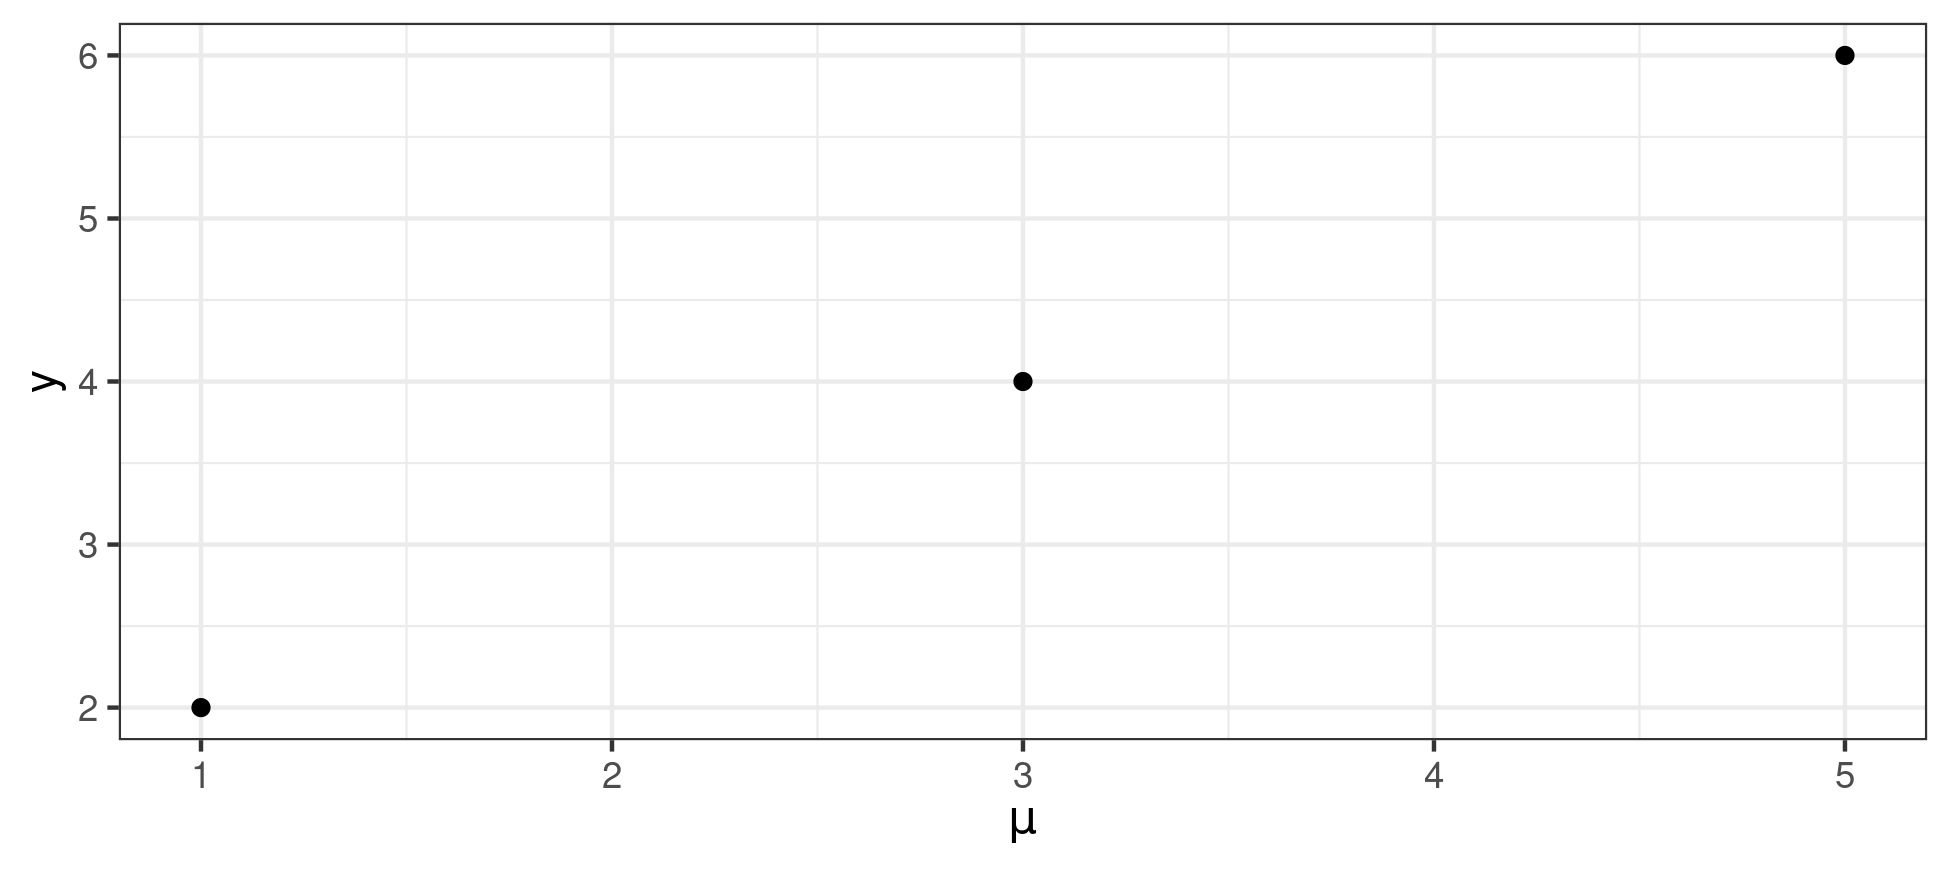
\includegraphics[width=0.98\linewidth,height=0.441\linewidth]{figure/exampleplot-1} 

}

\caption[]{Caption  here}\label{fig:exampleplot}
\end{figure}

\end{knitrout}
}



% %%%%%%%%%%%%%%%%%%%%%%

\newcommand{\ExampleTable}{

\begin{tabular}{r|r}
\hline
x & y\\
\hline
1 & 2\\
\hline
3 & 4\\
\hline
5 & 6\\
\hline
\end{tabular}

}

\DefineMacros{}

\title{Your Paper}
\author{You}

\begin{document}
\maketitle

\begin{abstract}
Your abstract.
\end{abstract}


\section{Introduction}
Most local Bayesian sensitivity analysis uses series expansions of
expectations.  Some problems:
%
\begin{itemize}
\item Can produce impossible posteriors (negative variances)
\item Some things depend on a large or infinite number of moments (quantiles, more complex functionals)
\item MCMC noise
\item People like draws not analytic expressions
\end{itemize}
%
So we do flows.  We particularly focus on approximating the bootstrap, though our methodology is
general.

\section{Knitr Example}

There are $\NumRows$ in the example.

\ExamplePlot{}

\ExampleTable{}


\clearpage
\bibliography{sample}

\end{document}
